% This is text associated with the open textbook "Open Electromagnetics"
% See immediately below for author, date
% This work is licensed under the Creative Commons Attribution-ShareAlike 4.0 International License. (CC BY-SA 4.0) 
% To view a copy of the license, visit http://creativecommons.org/licenses/by-sa/4.0/

%ORB TITLE Radiation from a Current Moment
%ORB AUTHOR 0        # S.W. Ellingson, Virginia Tech (ellingson@vt.edu)
%ORB DATE 20191123   # yyyymmdd
%ORB ABSTRACT 

\label{m0194_Radiation_Current_Moment} % <-- Must match name of this file and module directory name.  Don't mess with this!
%\index{optical fiber|(}

In this section, we begin to address the following problem:  
Given a distribution of impressed current density ${\bf J}({\bf r})$, what is the resulting electric field intensity ${\bf E}({\bf r})$?
One route to an answer is via Maxwell's equations.
\index{Maxwell's equations}
Viewing Maxwell's equations as a system of differential equations, a rigorous mathematical solution is possible given the appropriate boundary conditions.
The rigorous solution following that approach is relatively complicated, and is presented beginning in Section~\ref{m0195_Magnetic_Vector_Potential} of this book.

If we instead limit scope to a sufficiently simple current distribution, a simple informal derivation is possible.
This section presents such a derivation. 
The advantage of tackling a simple special case first is that it will allow us to quickly assess the nature of the solution, which will turn out to be useful once we do eventually address the more general problem.
Furthermore, the results presented in this section will turn out to be sufficient to tackle many commonly-encountered applications.

The simple current distribution considered in this section is known as a \emph{current moment}.
An example of a current moment is shown in Figure~\ref{m0194_fCurrentMoment} and in this case is defined as follows:
%
\begin{figure}[b!] % <--- "[b!]" for first figure in section *only*; delete for 2nd and subsequent figures
\begin{center}
\pdftooltip{{  % note double braces
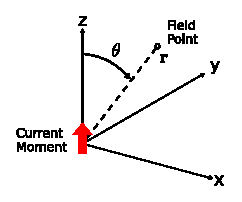
\includegraphics[width=2in]{modules/m0194_fCurrentMoment.eps} 
% https://commons.wikimedia.org/wiki/File:A_z-directed_current_moment_located_at_the_origin.svg
}}{An x-y-z Cartesian coordinate system with z vertical, x horizontal, and y into the page. For a field point labeled bold small r is an angle theta from the positive z axis. Thick arrow labeled “current moment” at the origin pointing up.}
\end{center}
\centerline{\scriptsize 
\copyright~\hyperref[m0194_fCurrentMoment_Credit]{C.\ Wang} 
\href{https://creativecommons.org/licenses/by-sa/4.0/}{CC BY-SA 4.0} 
} % \centerline 
\caption{
\label{m0194_fCurrentMoment}
A $+\hat{\bf z}$-directed current moment located at the origin.
}
\end{figure}
%
\begin{equation}
\Delta{\bf J}({\bf r}) = \hat{\bf z}~I~\Delta l~\delta({\bf r})
\label{m0194_eCM}
\end{equation}
%
where 
$I~\Delta l$ is the scalar component of the current moment, having units of current times length (SI base units of A$\cdot$m);
and $\delta({\bf r})$ is the volumetric sampling function\footnote{Also a form of the \emph{Dirac delta function};
\index{Dirac delta function} 
see ``Additional Reading'' at the end of this section.}
\index{sampling function}
defined as follows:
%
\begin{flalign}
~ &\delta({\bf r}) \triangleq 0~~~ \mbox{for}~~~ {\bf r}\neq 0;~~~ \mbox{and} \label{m0194_eDelta1} \\
~ &\int_{\mathcal{V}}\delta({\bf r})~dv \triangleq 1             \label{m0194_eDelta2}
\end{flalign}
%
where
$\mathcal{V}$ is any volume which includes the origin (${\bf r}=0$).
It is evident from Equation~\ref{m0194_eDelta2} that $\delta({\bf r})$ has SI base units of m$^{-3}$.
Subsequently, $\Delta{\bf J}({\bf r})$ has SI base units of A/m$^2$, confirming that it is a volume current density.
However, it is the \emph{simplest possible} form of volume current density, since -- as indicated by Equation~\ref{m0194_eDelta1} -- it exists only at the origin and nowhere else.
  
Although some current distributions approximate the current moment, current distributions encountered in common engineering practice generally do not exist in precisely this form.
Nevertheless, the current moment turns out to be generally useful as a ``building block'' from which practical distributions of current can be constructed, via the principle of superposition.
\index{superposition}
Radiation from current distributions constructed in this manner is calculated simply by summing the radiation from each of the constituent current moments. 

Now let us consider the electric field intensity $\Delta{\bf E}({\bf r})$ that is created by this current distribution.
First, if the current is steady (i.e., ``DC''), this problem falls within the domain of magnetostatics; i.e., the outcome is completely described by the magnetic field, and there can be no radiation.
Therefore, let us limit our attention to the ``AC'' case, for which radiation is possible. 
It will be convenient to employ phasor representation. 
In phasor representation, the current density is
%
\begin{equation}
\Delta\widetilde{\bf J}({\bf r}) = \hat{\bf z}~\widetilde{I}~\Delta l~\delta({\bf r})
\label{m0194_eCM2}
\end{equation}
%
where $\widetilde{I}~\Delta l$ is simply the scalar current moment expressed as a phasor.

Now we are ready to address the question ``What is $\Delta\widetilde{\bf E}({\bf r})$ due to $\Delta\widetilde{\bf J}({\bf r})$?''
Without doing any math, we know quite a bit about $\Delta\widetilde{\bf E}({\bf r})$.
For example:
%
\begin{itemize}
\item Since electric fields are proportional to the currents that give rise to them, we expect $\Delta\widetilde{\bf E}({\bf r})$ to be proportional to $\left|\widetilde{I}~\Delta l\right|$.
\item If we are sufficiently far from the origin, we expect $\Delta\widetilde{\bf E}({\bf r})$ to be approximately proportional to $1/r$ where $r\triangleq\left|{\bf r}\right|$ is the distance from the source current.  This is because point sources give rise to spherical waves, and the power density in a spherical wave would be proportional to $1/r^2$.
Since time-average power density is proportional to $\left|\Delta\widetilde{\bf E}({\bf r})\right|^2$, $\Delta\widetilde{\bf E}({\bf r})$ must be proportional to $1/r$.
\item If we are sufficiently far from the origin, and the loss due to the medium is negligible, then we expect the phase of $\Delta\widetilde{\bf E}({\bf r})$ to change approximately at rate $\beta$ where $\beta$ is the phase propagation constant $2\pi/\lambda$. Since we expect spherical phasefronts, $\Delta\widetilde{\bf E}({\bf r})$ should therefore contain the factor $e^{-j\beta r}$.  
\item Ampere's law 
\index{Ampere's law!general form}
indicates that a $\hat{\bf z}$-directed current at the origin should give rise to a $\hat{\bf \phi}$-directed magnetic field in the $z=0$ plane.\footnote{This is sometimes described as the ``right hand rule'' of Ampere's law.}  
At the same time, Poynting's theorem 
\index{Poynting's theorem}
requires the cross product of the electric and magnetic fields to point in the direction of power flow.
In the present problem, this direction is away from the source; i.e., $+\hat{\bf r}$.  Therefore, $\Delta\widetilde{\bf E}(z=0)$ points in the $-\hat{\bf z}$ direction.  The same principle applies outside of the $z=0$ plane, so in general we expect $\Delta\widetilde{\bf E}({\bf r})$ to point in the $\hat{\bf \theta}$ direction.
\item  
We expect $\Delta\widetilde{\bf E}({\bf r})=0$ along the $z$ axis.
Subsequently $\left|\Delta\widetilde{\bf E}(\hat{\bf r})\right|$ must increase from zero at $\theta=0$ and return to zero at $\theta=\pi$.
The symmetry of the problem suggests $\left|\Delta\widetilde{\bf E}(\hat{\bf r})\right|$ is maximum at $\theta=\pi/2$.
This magnitude must vary in the simplest possible way, leading us to conclude that $\Delta\widetilde{\bf E}(\hat{\bf r})$ is proportional to $\sin\theta$.
Furthermore, the radial symmetry of the problem means that $\Delta\widetilde{\bf E}(\hat{\bf r})$ should not depend at all on $\phi$.  
\end{itemize}
%
Putting these ideas together, we conclude that the radiated electric field has the following form:
%
\begin{equation}
\Delta\widetilde{\bf E}({\bf r}) \approx \hat{\bf \theta} C \left(\widetilde{I}~\Delta l\right) \left(\sin\theta\right) \frac{e^{-j\beta r}}{r}
\end{equation}
%
where $C$ is a constant which accounts for all of the constants of proportionality identified in the preceding analysis.
Since the units of $\Delta\widetilde{\bf E}({\bf r})$ are V/m, the units of $C$ must be $\Omega$/m.
We have not yet accounted for the wave impedance of the medium $\eta$, which has units of $\Omega$, so it would be a good bet based on the units that $C$ is proportional to $\eta$.
However, here the informal analysis reaches a dead end, so we shall simply state the result from the rigorous solution: $C=j\eta\beta/4\pi$.  The units are correct, and we finally obtain:
%
\begin{equation}
\Delta\widetilde{\bf E}({\bf r}) \approx \hat{\bf \theta} \frac{j\eta\beta}{4\pi} \left(\widetilde{I}~\Delta l\right) \left(\sin\theta\right)  \frac{e^{-j\beta r}}{r}
\end{equation}
%
Additional evidence that this solution is correct comes from the fact that it satisfies the wave equation 
$\nabla^2 \Delta\widetilde{\bf E}({\bf r}) + \beta^2 \Delta\widetilde{\bf E}({\bf r}) = 0$.\footnote{Confirming this is straightforward (simply substitute and evaluate) and is left as an exercise for the student.}

Note that the expression we have obtained for the radiated electric field is approximate (hence the ``$\approx$'').
This is due in part to our presumption of a simple spherical wave, which may only be valid at distances far from the source.
But how far?
An educated guess would be distances much greater than a wavelength (i.e., $r\gg\lambda$).
This will do for now; in another section, we shall show rigorously that this guess is essentially correct.

We conclude this section by noting that the current distribution analyzed in this section is sometimes referred to as a \emph{Hertzian dipole}.
\index{Hertzian dipole}
A Hertzian dipole is typically defined as a straight infinitesimally-thin filament of current with length which is very small relative to a wavelength, but not precisely zero.  
This interpretation does not change the solution obtained in this section,
thus we may view the current moment and the Hertzian dipole as effectively the same in practical engineering applications. 

%%%%%%%%%%%%%%%%%%%%%

{\bf Additional Reading:}
\begin{itemize}
\item ``\href{https://en.wikipedia.org/wiki/Dirac_delta_function}{Dirac delta function}'' on Wikipedia.
\item ``\href{https://en.wikipedia.org/wiki/Dipole_antenna#Hertzian_dipole}{Dipole antenna}'' (section entitled ``Hertzian Dipole'') on Wikipedia.
\end{itemize}

%\index{optical fiber|)}


